\documentclass[10pt,a4paper]{article}
\usepackage[utf8]{inputenc}
\usepackage{amsfonts}
\usepackage{graphicx}
\usepackage{subfig}
\graphicspath{ {images/} }
\usepackage{indentfirst}
\usepackage{float}
\usepackage{listings}

\lstset{
  basicstyle=\ttfamily,
  columns=fullflexible,
  frame=single,
  breaklines=true,
}

\begin{document}

\title{EncryptZip: \\ Compressed, Encrypted Containers on Android \\ Project Milestone}
\author{Alex Shah}
\date{4/7/18}

\maketitle

\section{Abstract}
This project sets out to implement encryption on zip based containers on the Android platform. This was accomplished with tools available in the Android SDK and Java. Containers are created by zipping a folder's contents on the user's device. Zipping a folder compresses it to save file size. A key is generated using SHA-256 from the user's provided password. The zipped container is then encrypted with AES using the generated key. These containers are thereby compressed, encrypted, and inherently portable.

\section{Introduction}

\subsection{Encryption}
Encrypting files is a common practice to prevent unauthorized or unintended access to sensitive information. However, encrypting each file is only one facet of security in a system. Encrypting a container which holds sensitive information can prove more useful than encrypting on a per file basis. This is especially useful in applications where the system cannot be entirely secured. It can also be used in addition to measures such as file and disk based encryption schemes. These three levels, file level, container level, and system/disk level encryption ensure that access is compartmentalized and can further secure a user's documents from unwanted access. 

\subsection{Compression}
By utilizing compression by zipping the contents of a directory, the container zip is only as large as its contents. In the mobile space this is especially important due to limitations in storage capacity and transmitting containers over a network.

\section{Background}

\subsection{Containers}
While desktop operating systems have applications to create encrypted containers, such as Veracrypt, Android does not have a native implementation. There are third party means, however these implementations use proprietary methods. In addition, solutions such as Veracrypt create fixed sized containers regardless of the size of the contents of the container. The goal of this project is to use built in features and standard systems to create a container level encryption scheme on the Android mobile platform which solves these problems.

\subsection{Solutions}
Zipping a directory creates a container no larger than its contents. By using zip compression, this solves the problem that Veracrypt and other third party implementations have, that the container does not remain a fixed size. Adding and removing documents from the container requires no resizing. The zip and and encryption methods work regardless of the files present in the container, including text, image, and video files.

\section{Methodology}
\subsection{Zip Implementation}
Utilizing the Android SDK and available cryptography libraries provided by Google and Java, it is feasible to implement both the zip and encryption methods to secure the files on an Android device. The zip methods were accomplished using java.io and java.zip libraries wherein the users documents are gathered in a file list, then using a zip output stream, are written to the zip path. 

\subsection{Encryption Implementation}
Using buttons and on click listener from Android Studio's tools, a use provides a password in the password field. When the encrypt button is pressed, the provided password is read in to be used as a key for encryption. A key is generated using SHA-256 with the provided password. This was accomplished with javax.crypto and java.security libraries. From the javax.crypto library we use AES with the key to encrypt a byte stream of the zip contents. This allows us to pass in the zip as a byte[] in order to impartially process the contents of the archive. The resulting encrypted file is unreadable without first being decrypted by the reverse procedure. The forward and reverse methods are robust at preventing accidental damage to the archive. The encrypted zip is not affected by incorrect decryption attempts. As an added precaution, the encryption step must use a password. Providing no password would either be insecure or at worst a randomly generated key would not be able to be decrypted, and the contents of the container would be lost. 

\section{Experiments}
To implement directory zipping in Android it was necessary to use a buffer to prevent bottlenecks. For example:

\begin{lstlisting}[language=Java]
fileOutputStream = new FileOutputStream(file);
zipOutputStream = new ZipOutputStream(new BufferedOutputStream(fileOutputStream));

byte data[] = new byte[BUFFER_SIZE];
FileInputStream fileInputStream = new FileInputStream(file.getPath());
input = new BufferedInputStream(fileInputStream, BUFFER_SIZE);
entryPath = file.getAbsolutePath().replace(parentPath, "");
ZipEntry entry = new ZipEntry(entryPath);
zipOutputStream.putNextEntry(entry);
int count;
while ((count = input.read(data, 0, BUFFER_SIZE)) != -1) {
  zipOutputStream.write(data, 0, count);
}
input.close();

\end{lstlisting}

It is necessary to use some additional libraries. These include security and extension libraries separate from the base Java libraries. These include:

\begin{lstlisting}[language=Java]
import java.security.NoSuchAlgorithmException;
import java.security.spec.InvalidKeySpecException;
import java.security.spec.KeySpec;
import javax.crypto.Cipher;
import javax.crypto.spec.PBEKeySpec;
\end{lstlisting}

These enable us to securely generate a 256 bit key using the provided password as well as encrypt the zip using AES with a 256 bit key, better than AES at 128 bits, and greater key length than what our in class implementation allowed.

In order to encrypt the zip, javax crypto and java security libraries are used in accordance to Android's security guidelines to perform SHA 256 and AES using a 256 bit key.

\clearpage

\begin{lstlisting}[language=Java]
// generate key from password using AES
    public static SecretKey generateKey(char[] password) throws NoSuchAlgorithmException, InvalidKeySpecException {
        final int iterations = 1000;

        // Generate a 256-bit key with SHA256
        final int outputKeyLength = 256;
        byte[] salt = new byte[20];

        SecretKeyFactory secretKeyFactory = SecretKeyFactory.getInstance("PBKDF2withHmacSHA256");
        KeySpec keySpec = new PBEKeySpec(password, salt, iterations, outputKeyLength);
        SecretKey secretKey = secretKeyFactory.generateSecret(keySpec);
        return secretKey;
    }

    // encrypt with AES
    public static byte[] encrypt(SecretKey key, byte[] fileData) throws Exception {
        Cipher cipher = Cipher.getInstance("AES");
        cipher.init(Cipher.ENCRYPT_MODE, key);
        byte[] encrypted = cipher.doFinal(fileData);
        return encrypted;
    }

\end{lstlisting}

\clearpage

\section{App}

\subsection{UI}

The main screen of the EncryptZip app. The zip, unzip, encrypt, and decrypt buttons use on click listeners to perform their named functions.

\begin{figure}[H]
\centering
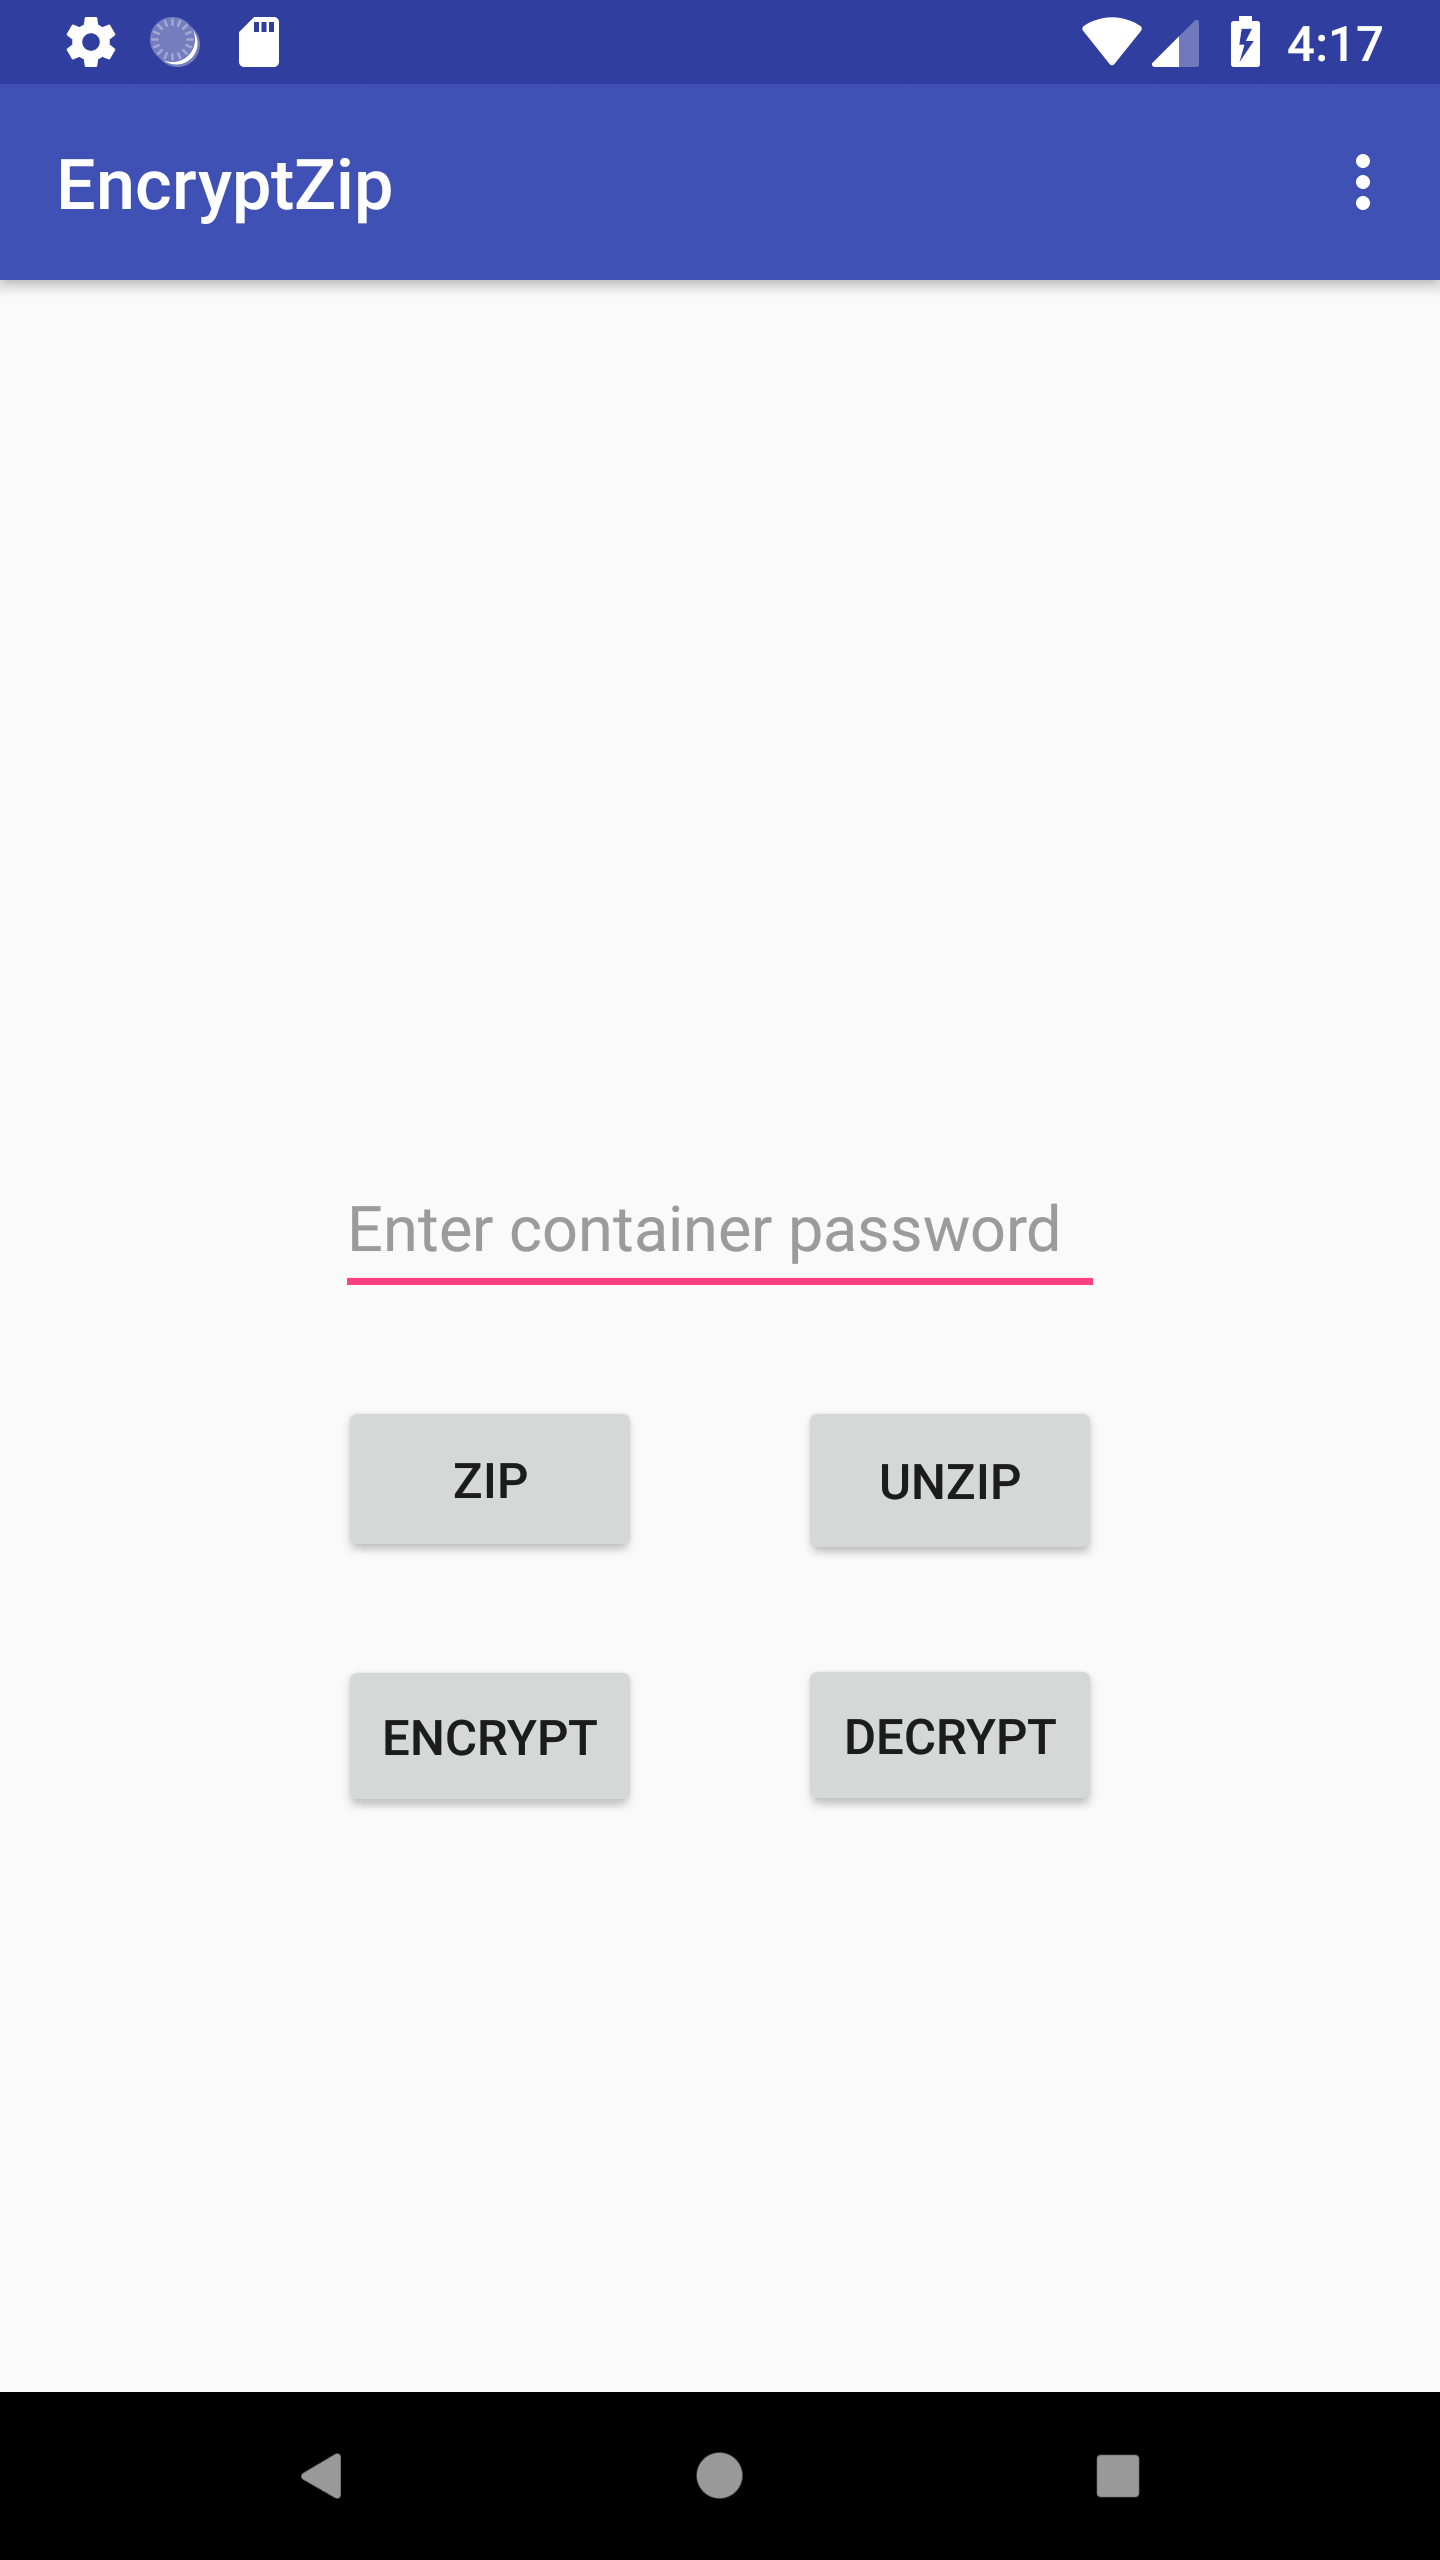
\includegraphics[width=9.5cm]{main1}
\caption{EncryptZip Main Screen}
\end{figure}

\clearpage

Toast notifications are shown to the user to indicate whether an action has completed successfully or not.
\begin{figure}
    \centering
    \subfloat[Success!]{{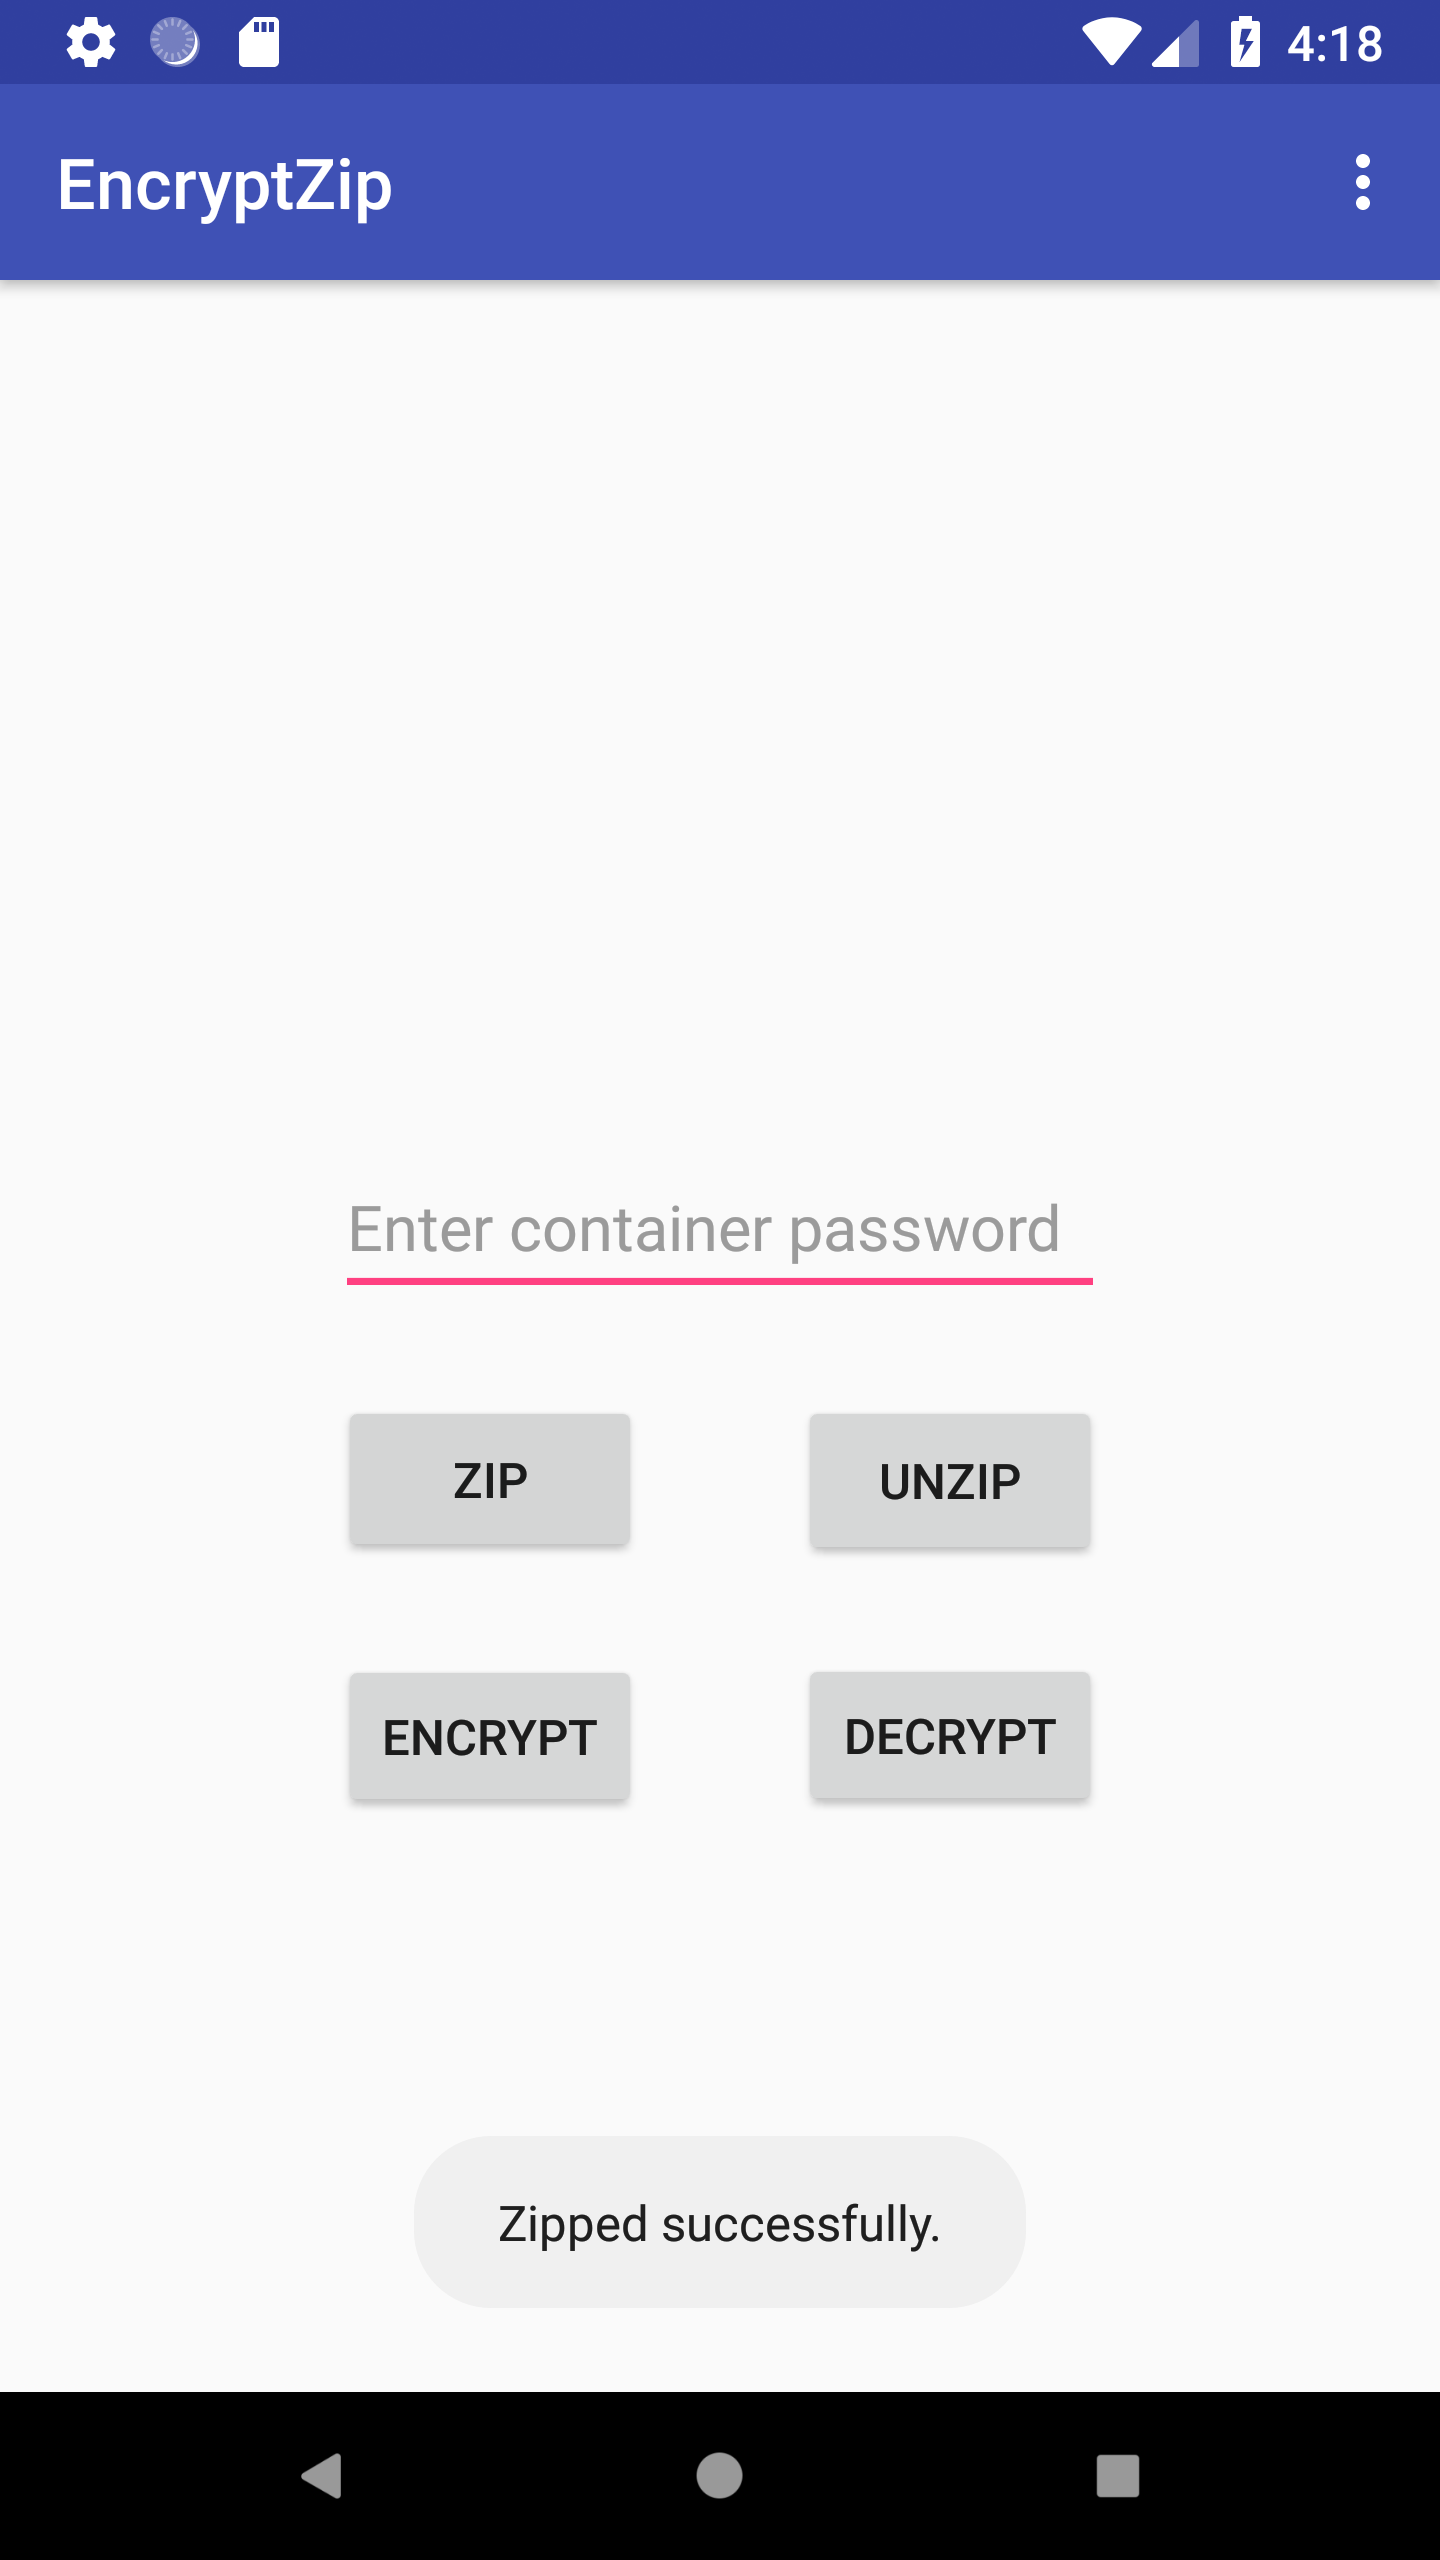
\includegraphics[width=5cm]{toast1} }}
    \qquad
    \subfloat[Failure]{{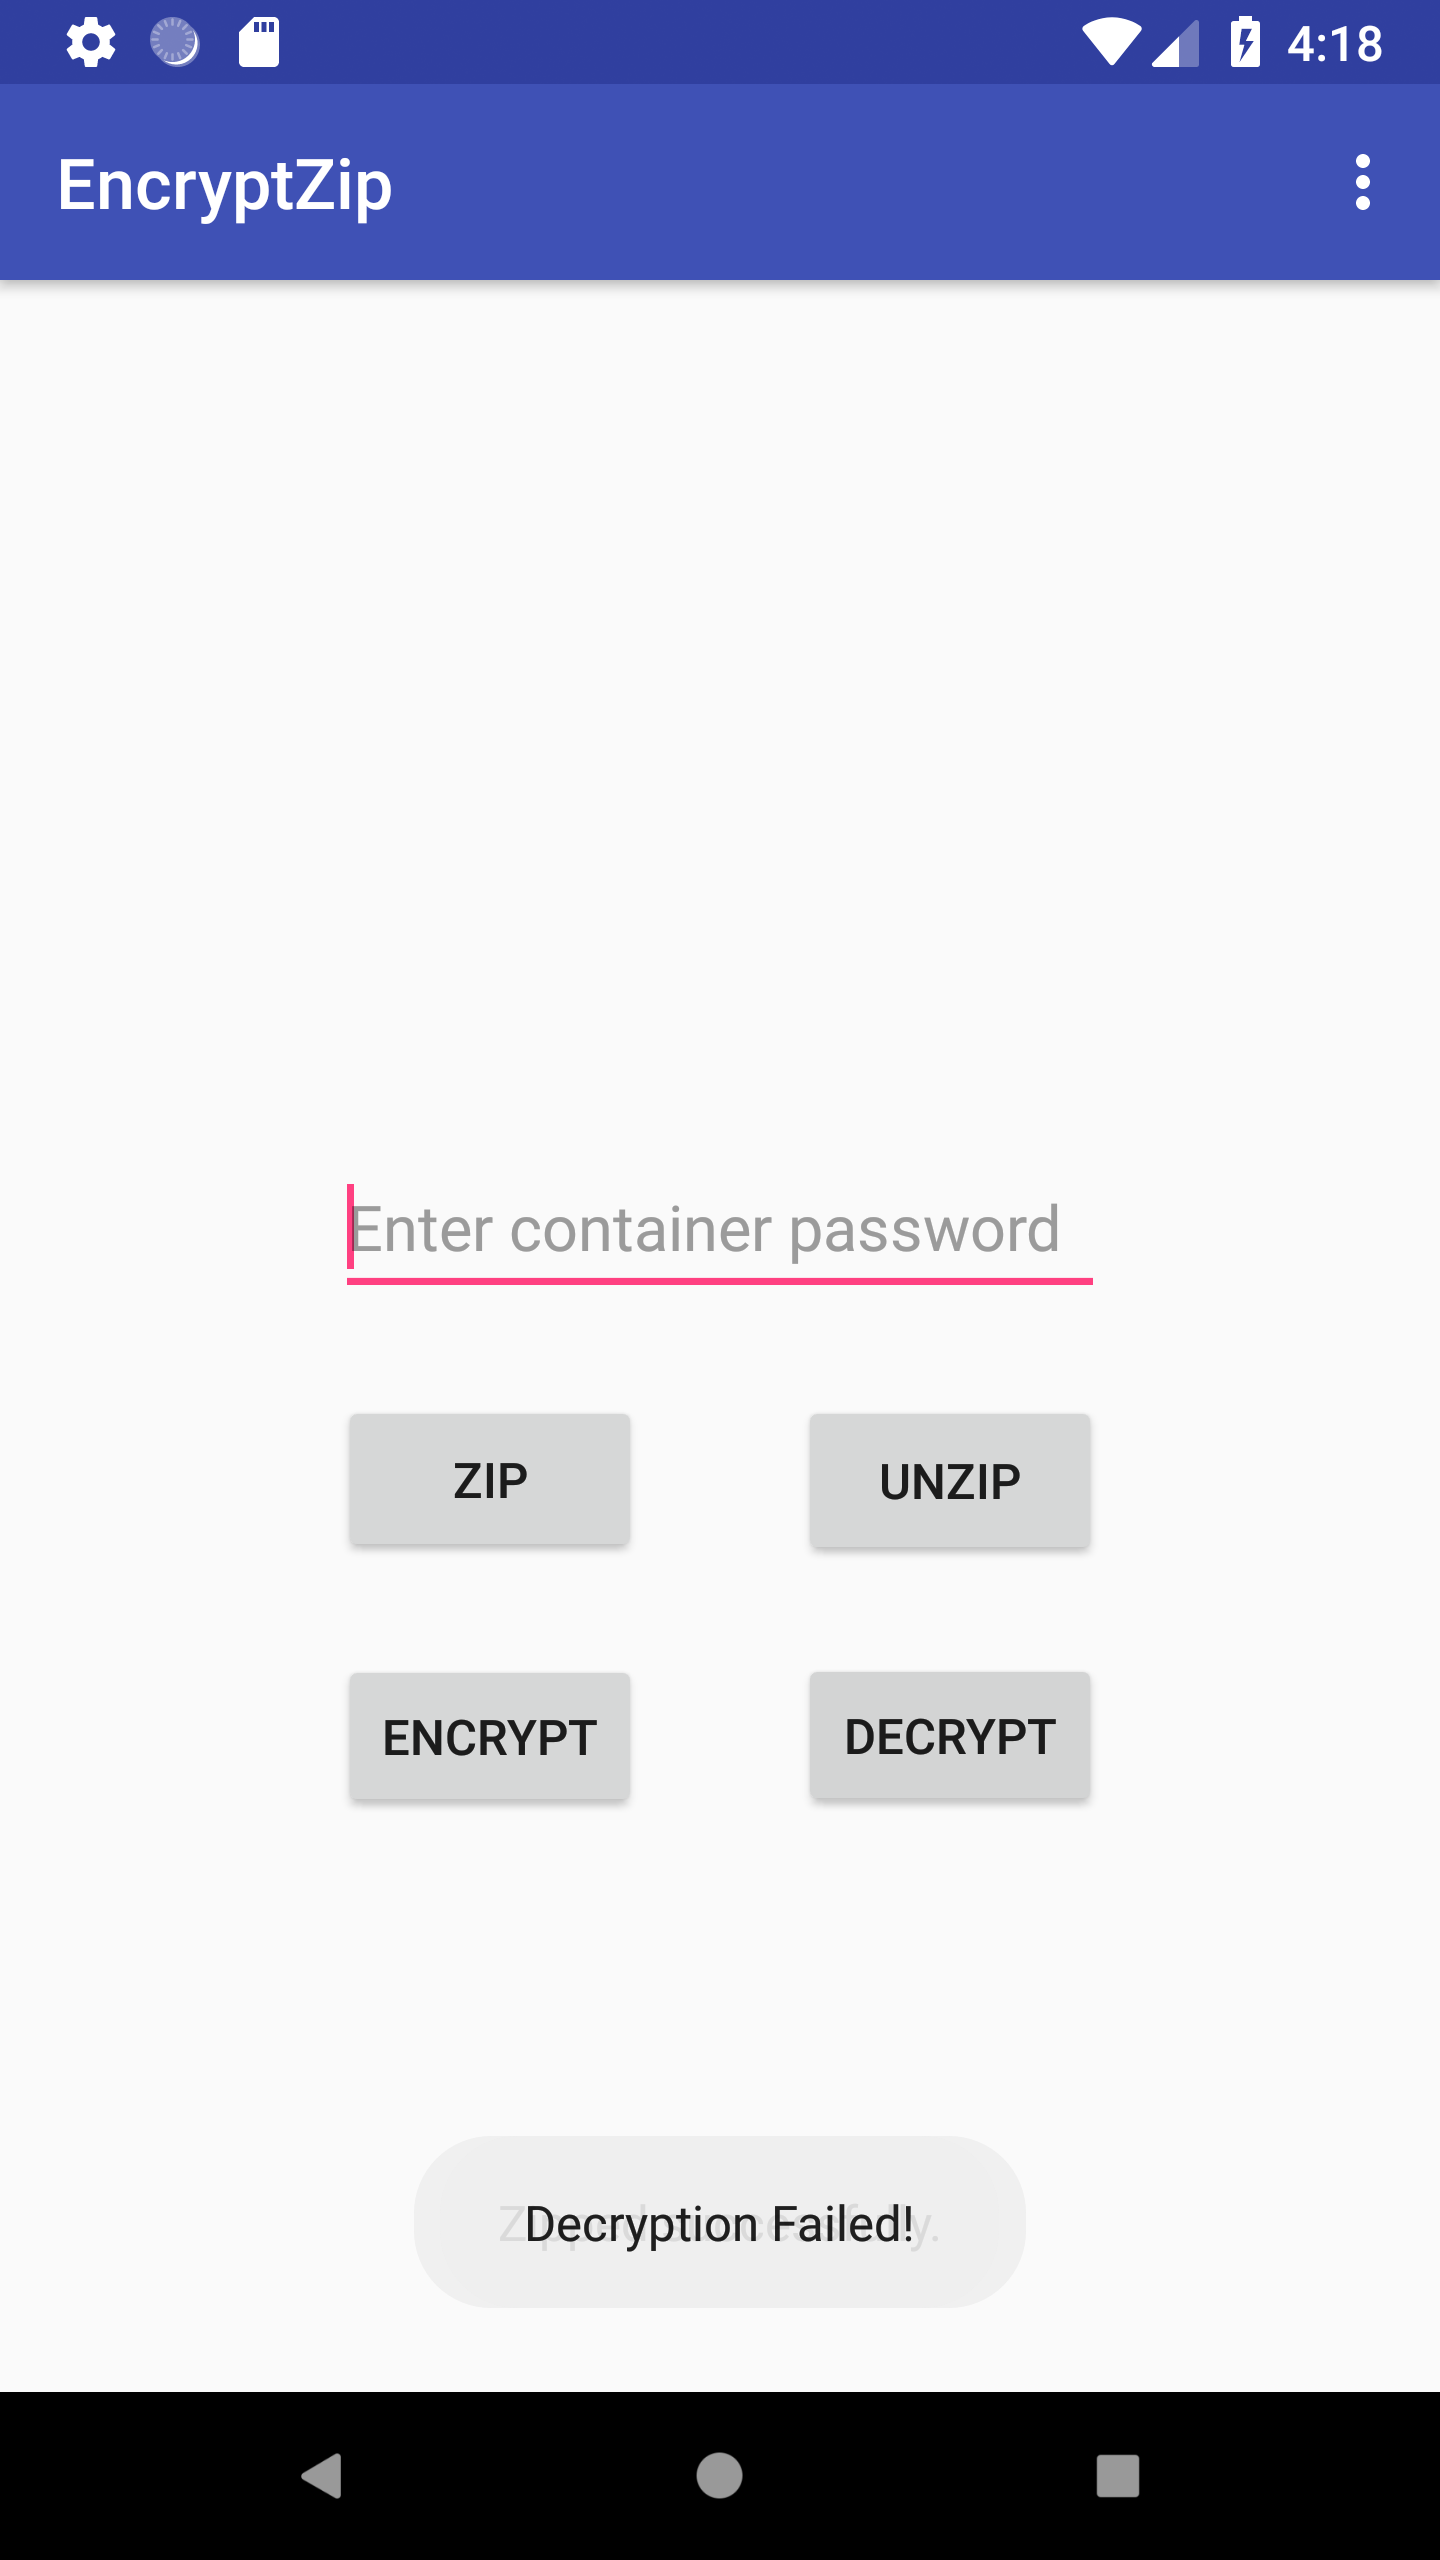
\includegraphics[width=5cm]{toast2} }}
    \caption{Toast Notifications}
    \label{fig:toast}
\end{figure}

\clearpage

The data folder is accessible through the file system on Android devices. The contents of the data folder are zipped and the resulting zip file is stored in the zip folder.
\begin{figure}[H]
\centering
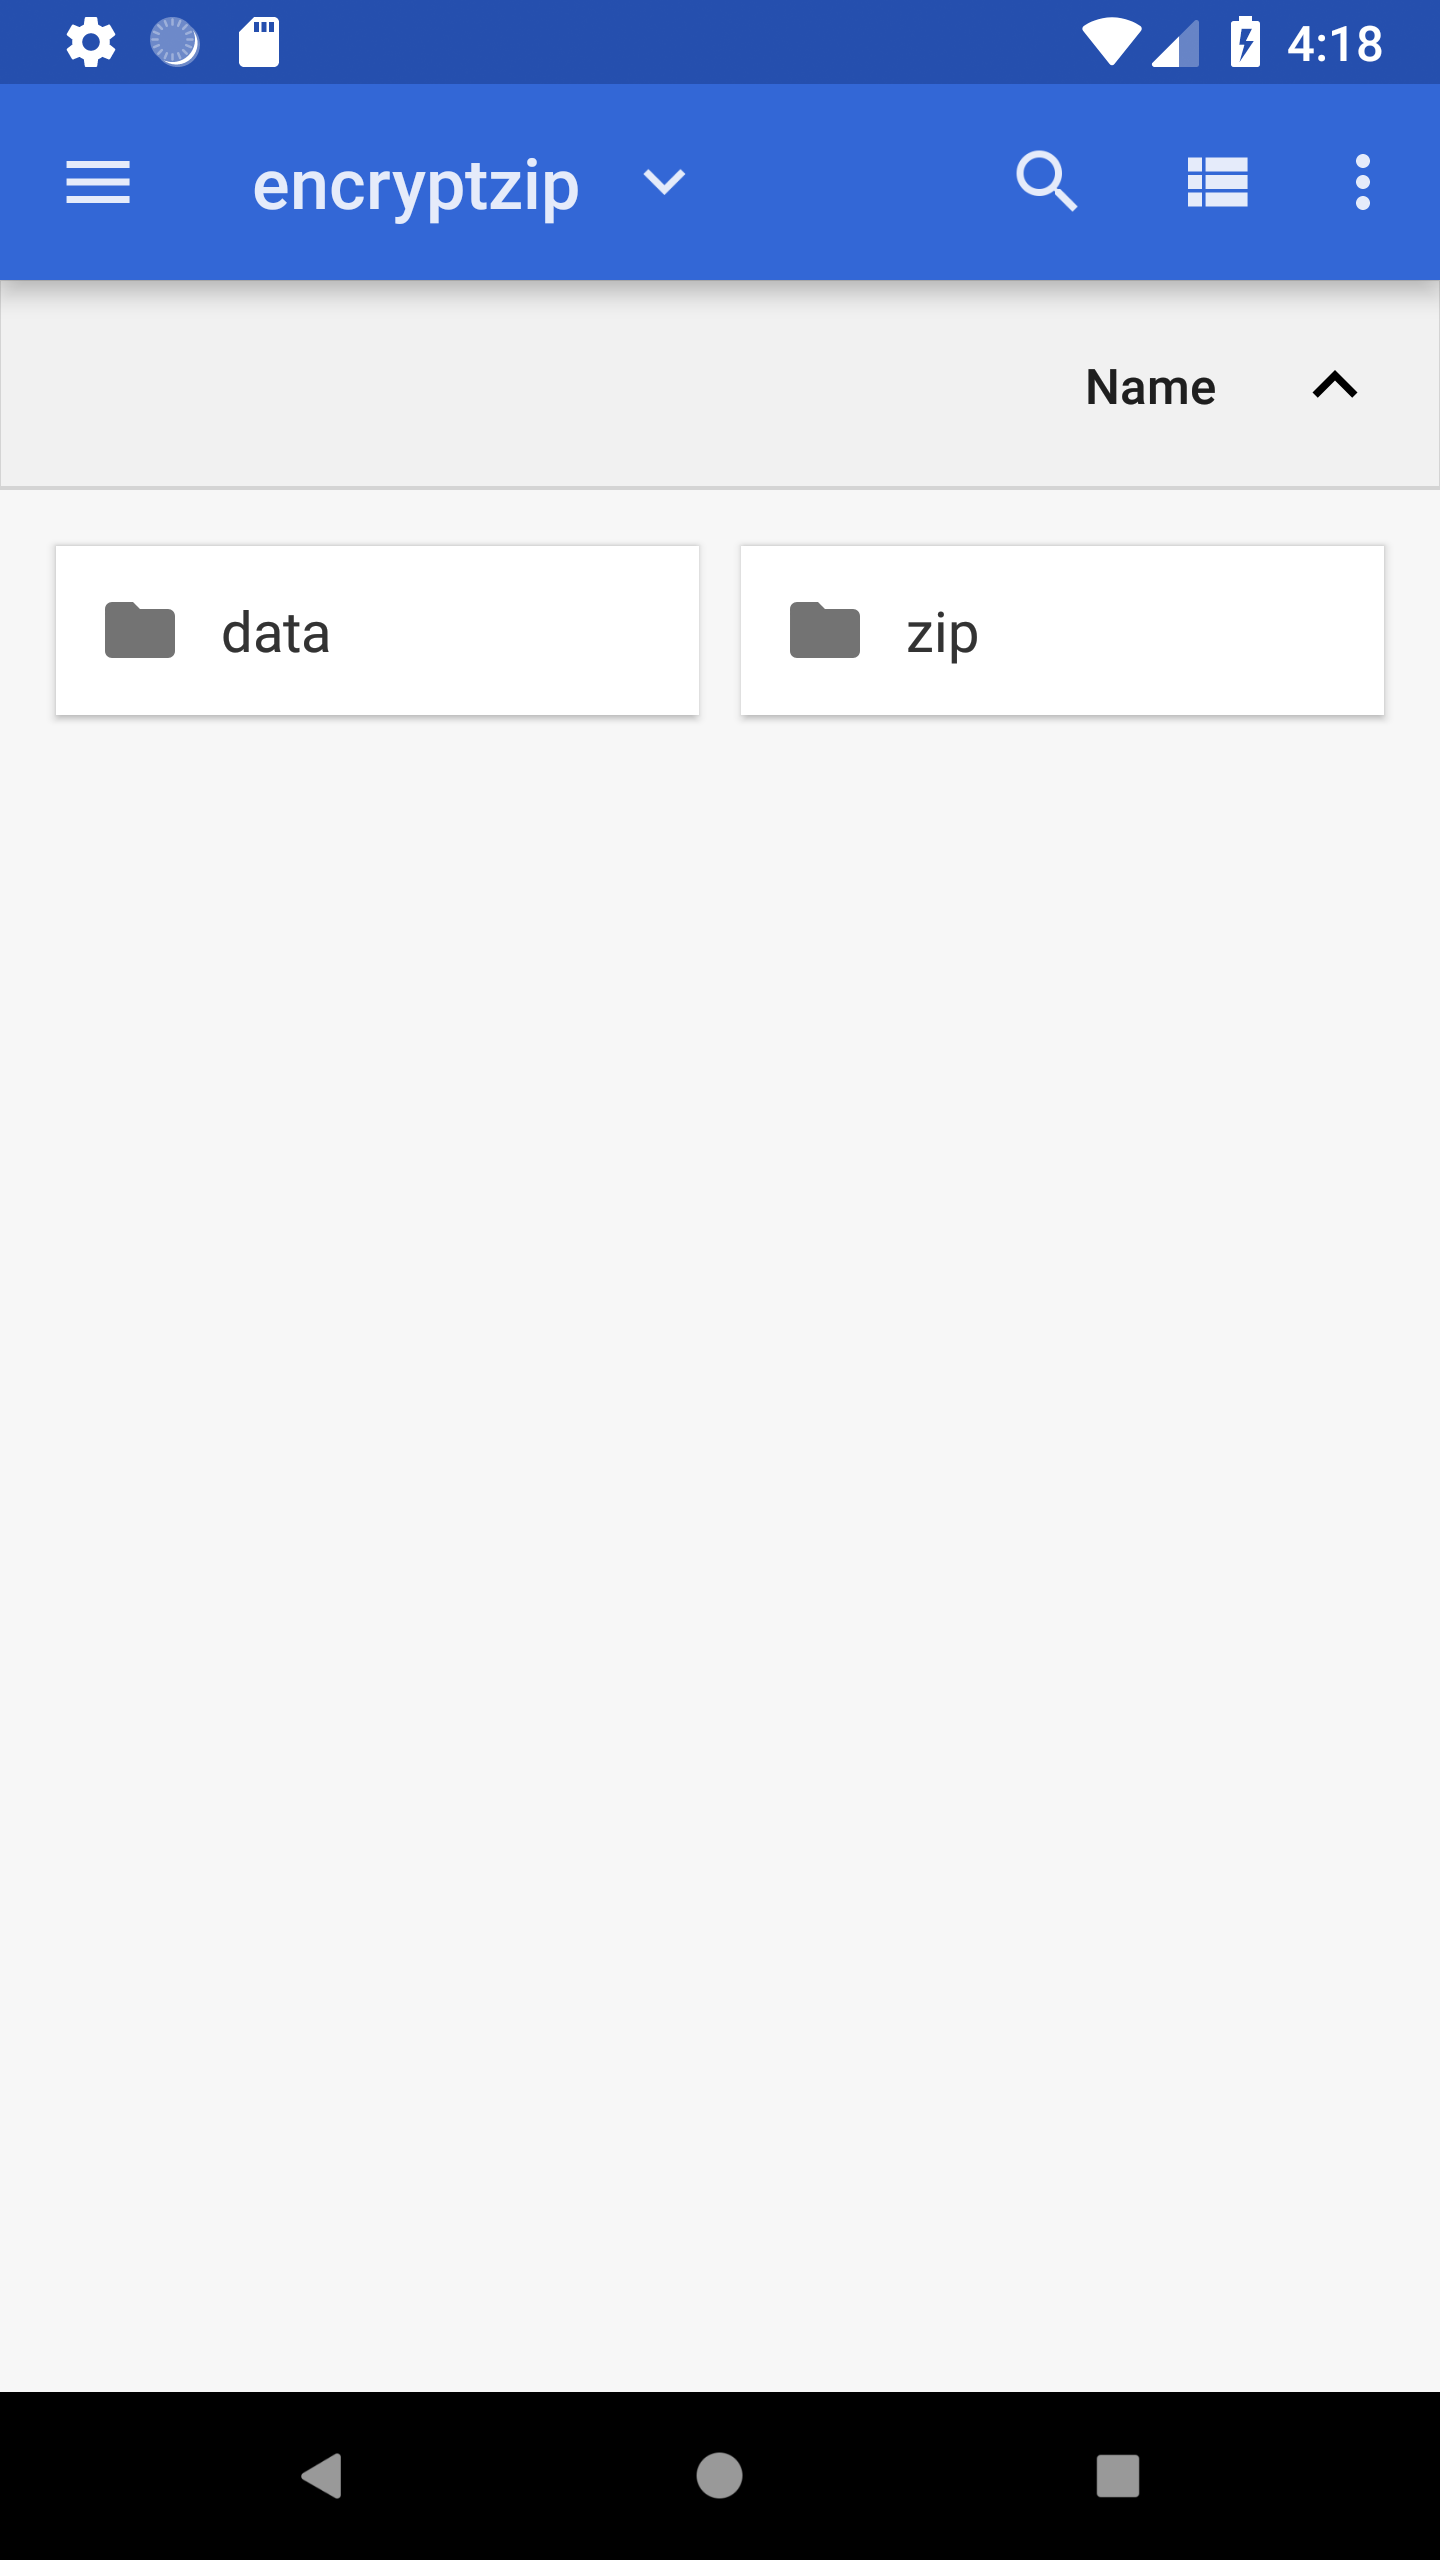
\includegraphics[width=8cm]{file1}
\caption{File System}
\end{figure}

\clearpage

\subsection{Main Flow}

\begin{figure}[H]
\centering
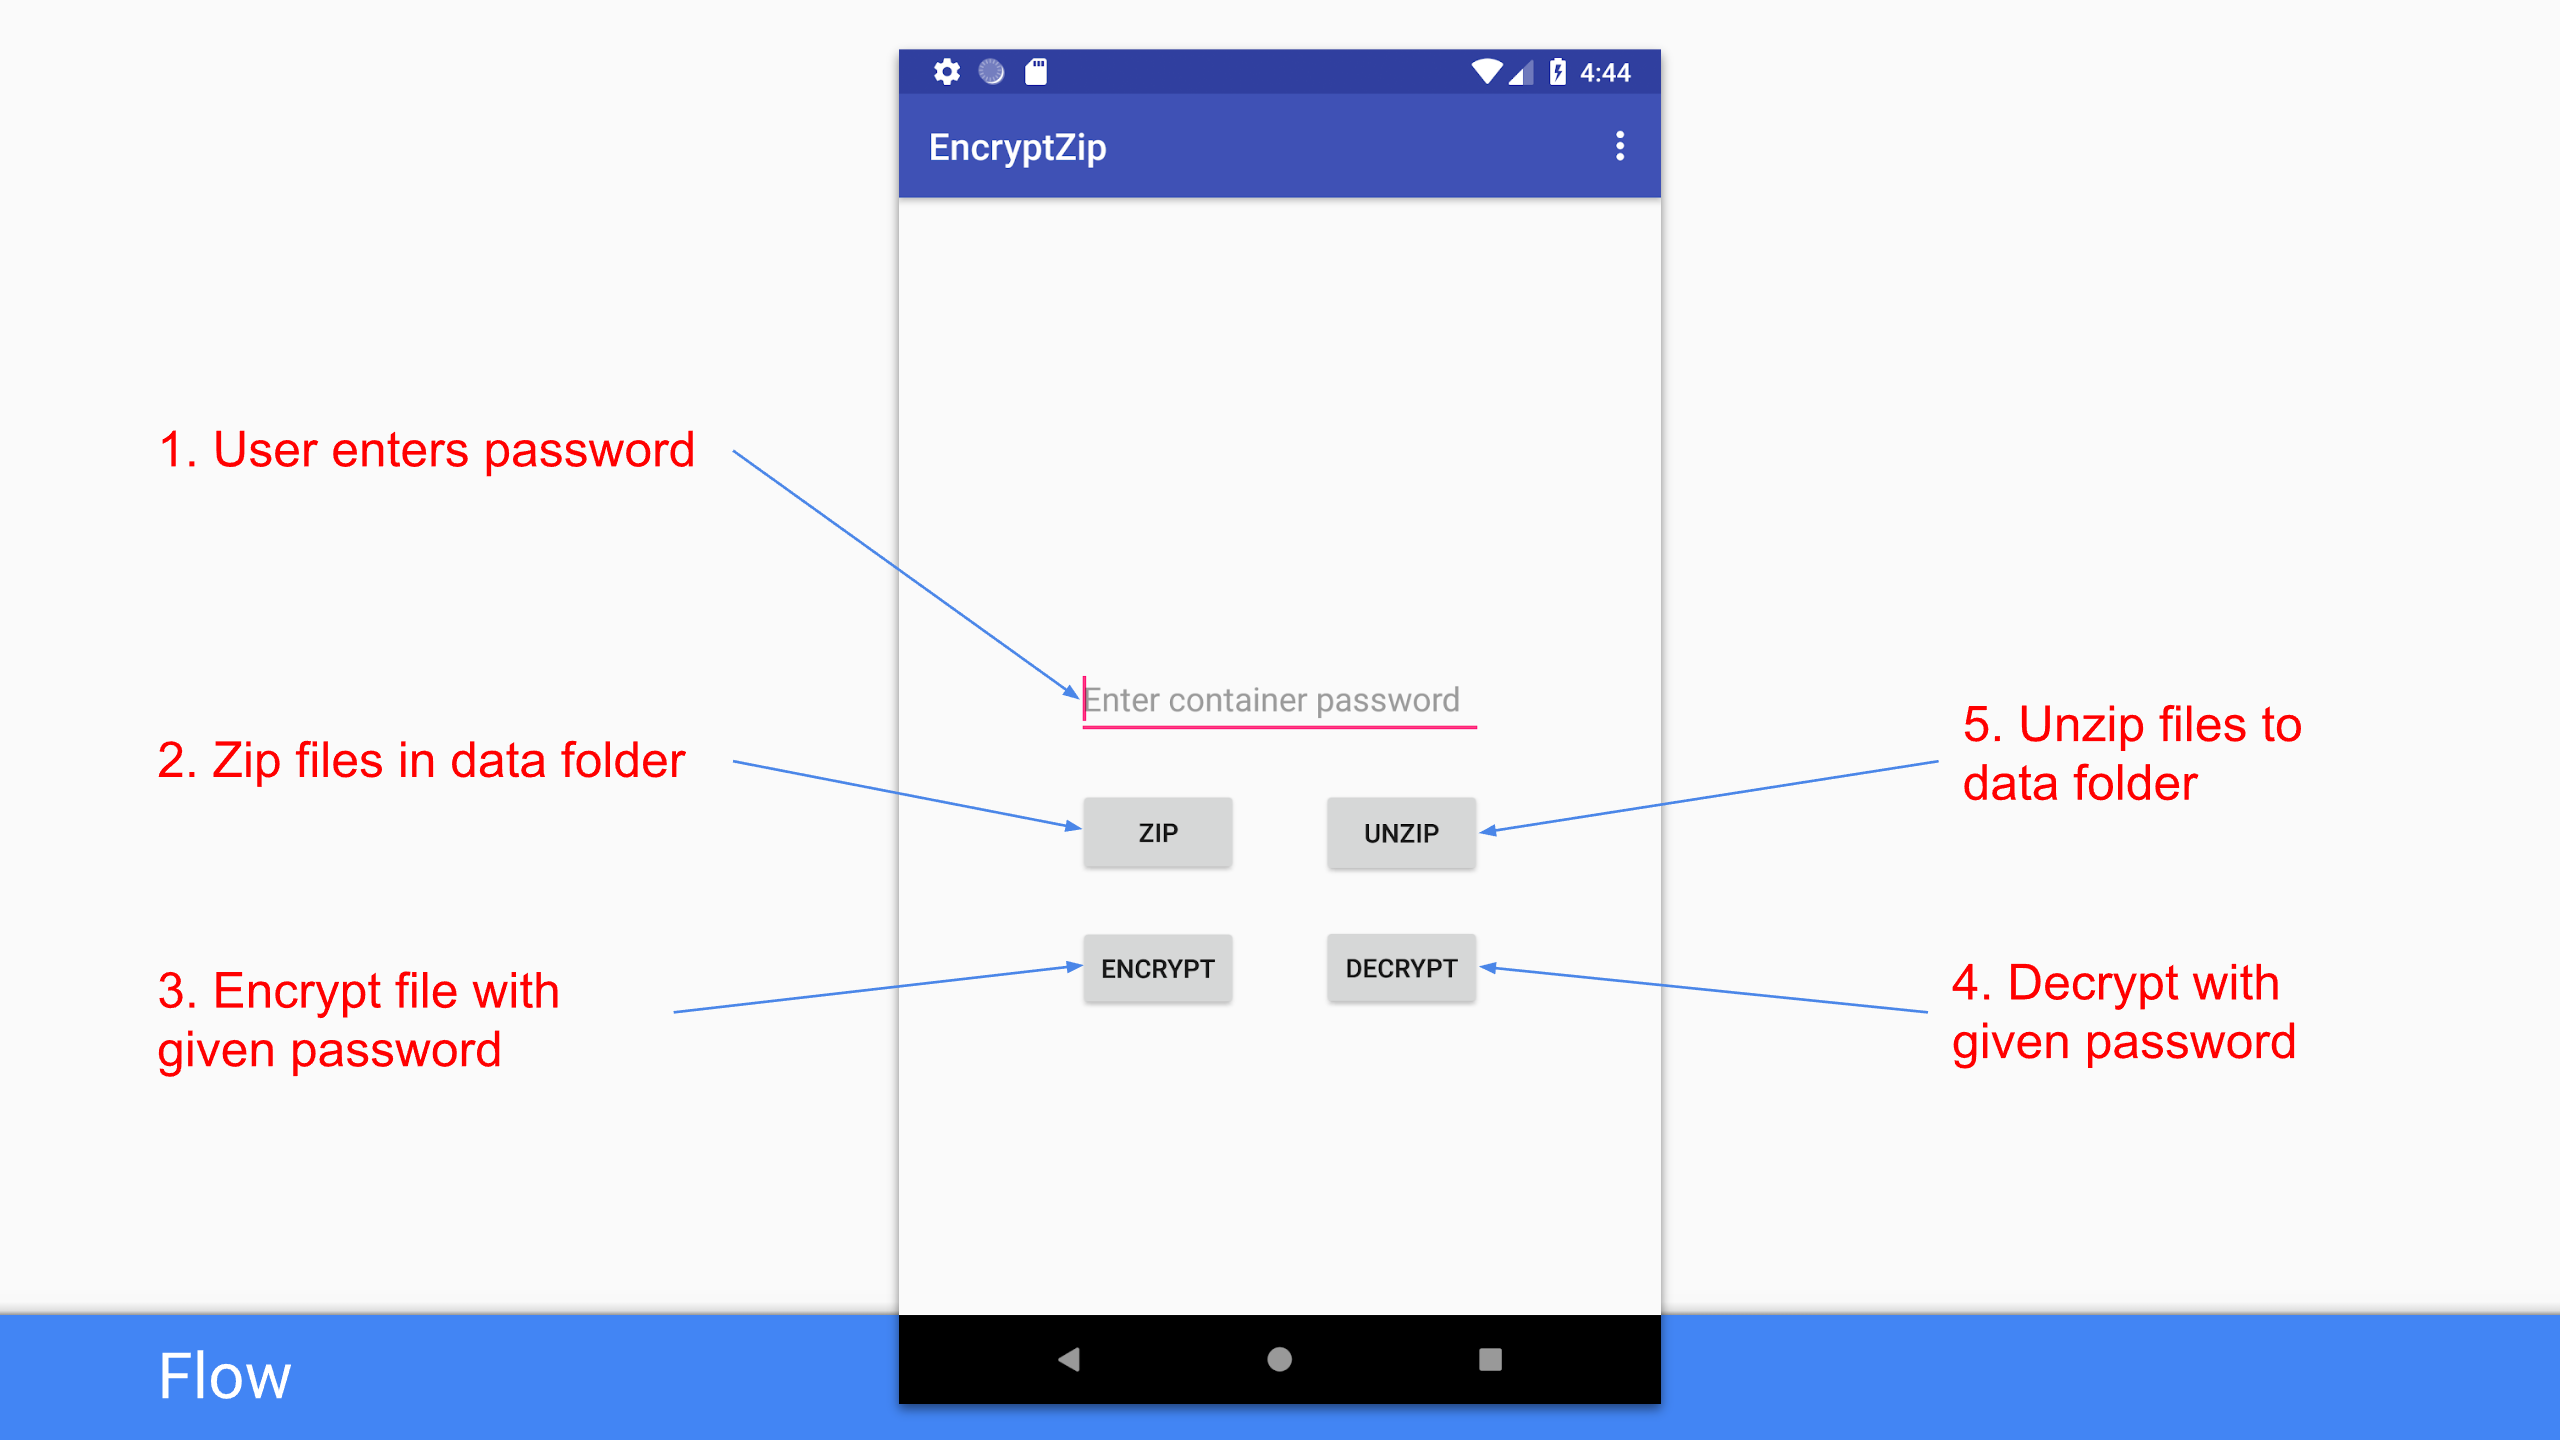
\includegraphics[width=\textwidth]{flow1}
\caption{EncryptZip Flow}
\end{figure}

\section{Conclusion}
The project was a success. The contents of the Android directory are fully processed by the zip and unzip functions. The resulting zip files are able to be successfully encrypted and decrypted with a given key. The encryption scheme exceeds the requirements, using SHA 256 and AES with a 256 bit key. 

\section{Sources}

 “Meet Android Studio  |  Android Developers.” Android Developers, developer.android.com/studio/intro/index.html.
\\

“Package Java.security.” 28 Mar. 2018, docs.oracle.com/javase/8/docs/api/java/security/package-summary.html.
\\

“Package Javax.crypto.” 28 Mar. 2018, docs.oracle.com/javase/8/docs/api/javax/crypto/package-summary.html. 

\end{document}